\section{Experiments and results} \label{experimental_setup}

%\subsection{Evaluation datasets}
%\label{experimental_setup:A}

The proposed BrainGNN is evaluated on two datasets. On the one hand the Biopoint Autism Study Dataset (Biopoint) \cite{Venkataraman2016BayesianCD} is used. It deals with a binary prediction task, whether a patient has autism or not. On the other hand the Human Connectome Project (HCP) 900 Subject Release dataset \cite{VANESSEN201362} is used. The task is a multi class classification, to distinguish between different tasks (e.g. motorical task, language task, gambling). For details about the datasets, please refer to  \cite{Venkataraman2016BayesianCD} and \cite{VANESSEN201362}.

%\subsection{Prediction results}
%\label{experimental_setup:B}

Table \ref{fig:prediction_results} shows the prediction results of BrainGNN in comparison to other approaches. For both datasets, BrainGNN outperforms all other approaches.

\begin{figure}[ht]
	\centering
	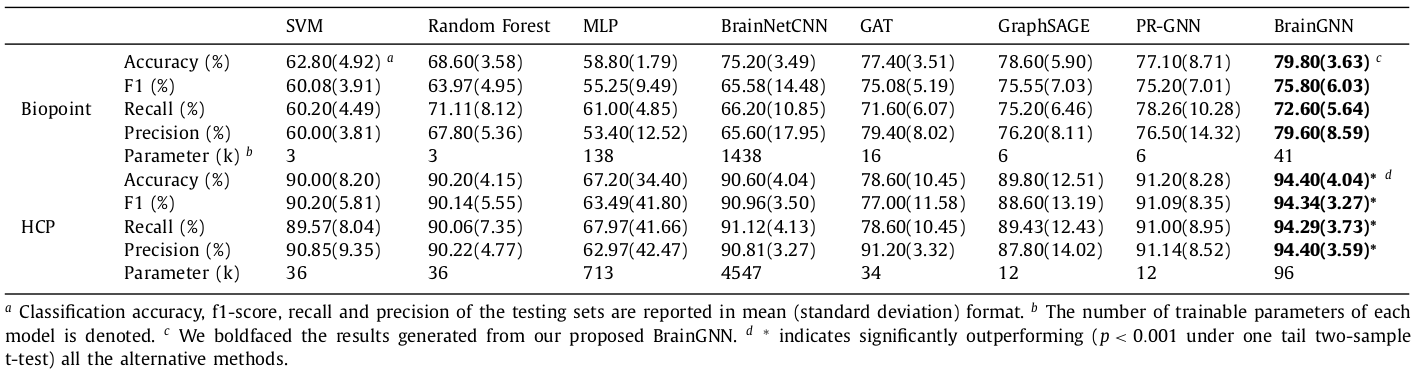
\includegraphics[width=1.0\linewidth]{figures/predictionResults.png}
	\caption{Prediction results of BrainGNN compared to other baseline approaches}
	\cite{LI2021102233}
	\label{fig:prediction_results}
\end{figure}

%\subsection{Interpretation results}
%\label{experimental_setup:C}

Besides the classification, the interpretation of the results is also possible.
On the one hand, the detection of biomarkers is possible. For both datasets the detected biomarkers are validated by literature. 
On the other hand the detected brain community patterns can be interpreted.
For a detailed description of the interpretation process, please refer to \cite{LI2021102233}.
